%%%%%%%%%%%%%%%%%%%%%%%%%%%%%%%%%%%%%%%%%
% baposter Portrait Poster
% LaTeX Template
% Version 1.0 (15/5/13)
%
% Created by:
% Brian Amberg (baposter@brian-amberg.de)
%
% This template has been downloaded from:
% http://www.LaTeXTemplates.com
%
% License:
% CC BY-NC-SA 3.0 (http://creativecommons.org/licenses/by-nc-sa/3.0/)
%
%%%%%%%%%%%%%%%%%%%%%%%%%%%%%%%%%%%%%%%%%

%----------------------------------------------------------------------------------------
%	PACKAGES AND OTHER DOCUMENT CONFIGURATIONS
%----------------------------------------------------------------------------------------

\documentclass[archE1,portrait]{baposter}

%841mm x 1189mm
\usepackage[font=small,labelfont=bf]{caption} % Required for specifying captions to tables and figures
\usepackage{booktabs} % Horizontal rules in tables
\usepackage{relsize} % Used for making text smaller in some places
\usepackage[urlcolor  = blue]{hyperref}
\graphicspath{{figures/}} % Directory in which figures are stored

\definecolor{bordercol}{RGB}{5,2,82} % Border color of content boxes
\definecolor{headercol1}{RGB}{5,2,82} % Background color for the header in the content boxes (left side)
\definecolor{headercol2}{RGB}{5,2,82} % Background color for the header in the content boxes (right side)
\definecolor{headerfontcol}{RGB}{255,255,255} % Text color for the header text in the content boxes
\definecolor{boxcolor}{RGB}{255,255,255} % Background color for the content in the content boxes

\begin{document}

\background{ % Set the background to an image (background.pdf)

}

\begin{poster}{
grid=false,
borderColor=bordercol, % Border color of content boxes
headerColorOne=headercol1, % Background color for the header in the content boxes (left side)
headerColorTwo=headercol1, % Background color for the header in the content boxes (right side)
headerFontColor=headerfontcol, % Text color for the header text in the content boxes
boxColorOne=boxcolor, % Background color for the content in the content boxes
headershape=roundedright, % Specify the rounded corner in the content box headers
headerfont=\Large\sf\bf, % Font modifiers for the text in the content box headers
textborder=rectangle,
background=user,
headerborder=open, % Change to closed for a line under the content box headers
boxshade=plain
}
{}
%
%----------------------------------------------------------------------------------------
%	TITLE AND AUTHOR NAME
%----------------------------------------------------------------------------------------
%
%\vspace{2em}
{
%\newline
\sf\bf MoCA : Tool for \underline{M}otif \underline{C}onservation \underline{A}nalysis} % Poster title
{\vspace{1em} Saket Choudhary, Anton Valouev\\ % Author names
{\smaller \{skchoudh, valouev\}@usc.edu}\\
%\vspace{1em}
\underline{\url{http://moca.usc.edu}}
%\vspace{1em}
} % Author email addresses
%

%----------------------------------------------------------------------------------------
%	INTRODUCTION
%----------------------------------------------------------------------------------------

\headerbox{Introduction}{name=introduction,column=0,row=0, span=3}{
\begin{itemize}
\item Motifs are Short DNA sequences that appear recurrently and often  act as sequence specific binding sites for transcription factors
\item  Determining the quality of a reported ChIP-Seq motif is hard
\item  Motif analysis tools such as MEME\cite{bailey2015meme} can often report `false motifs' and still have significant p-value(or E-values)
\item `Distance from center' approach fails to identify new co-transcription factor motifs
\end{itemize}

}

%\headerbox{True vs False Motifs}{name=introduction2,column=1,row=0, span=2}{
%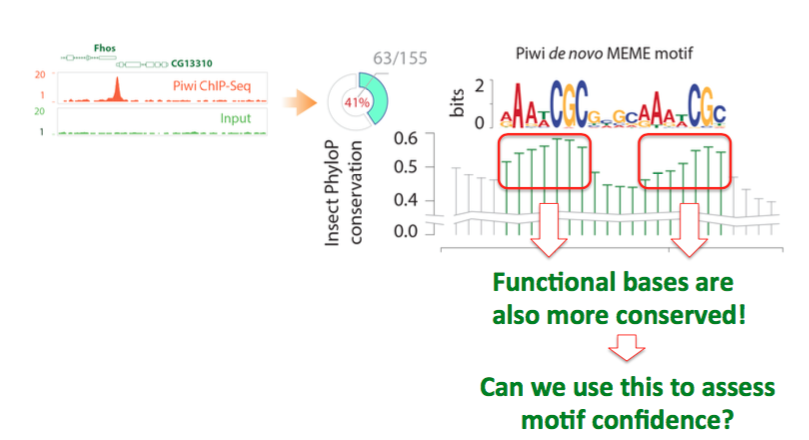
\includegraphics[scale=0.42]{motif_study}
%}

%----------------------------------------------------------------------------------------
%	MATERIALS AND METHODS
%----------------------------------------------------------------------------------------

\headerbox{Materials and Methods}{name=methods,column=0,below=introduction, span=3}{


\underline{\textbf{Hypothesis}}
\begin{itemize}
\item `True' transcription factor(TF) motifs have significant correlation between motif and conservation
\item `True' TF motifs have higher conservation scores at motif bases as compared to flanking bases
\end{itemize}


\underline{\textbf{MoCA}}

\begin{itemize}
\item Any metric to assess the quality of motifs, should also rely on biological relevance besides the statistical analysis
\item Since the motif acts as a specific binding sequence, it can be expected to be conserved evolutionarily
\item MoCA makes use of the PhyloP and Gerp scores to assess the conservation profile 
\item Automated analysis of ENCODE datasets, with a RESTful api
\end{itemize}

}



%----------------------------------------------------------------------------------------
%	REFERENCES
%----------------------------------------------------------------------------------------










%----------------------------------------------------------------------------------------
%	RESULTS
%----------------------------------------------------------------------------------------
\headerbox{Conclusions}{name=conclusion,span=1,column=2,below=methods}{
\begin{itemize}
\item MoCA is a helpful tool for identifying `true' motifs
\item MoCA's RESTful api allows automated analysis of ENCODE ChIP-seq datasets 
\end{itemize}
}
\headerbox{Results}{name=results2,span=2,column=0,below=methods}{ 



%------------------------------------------------

\begin{center}
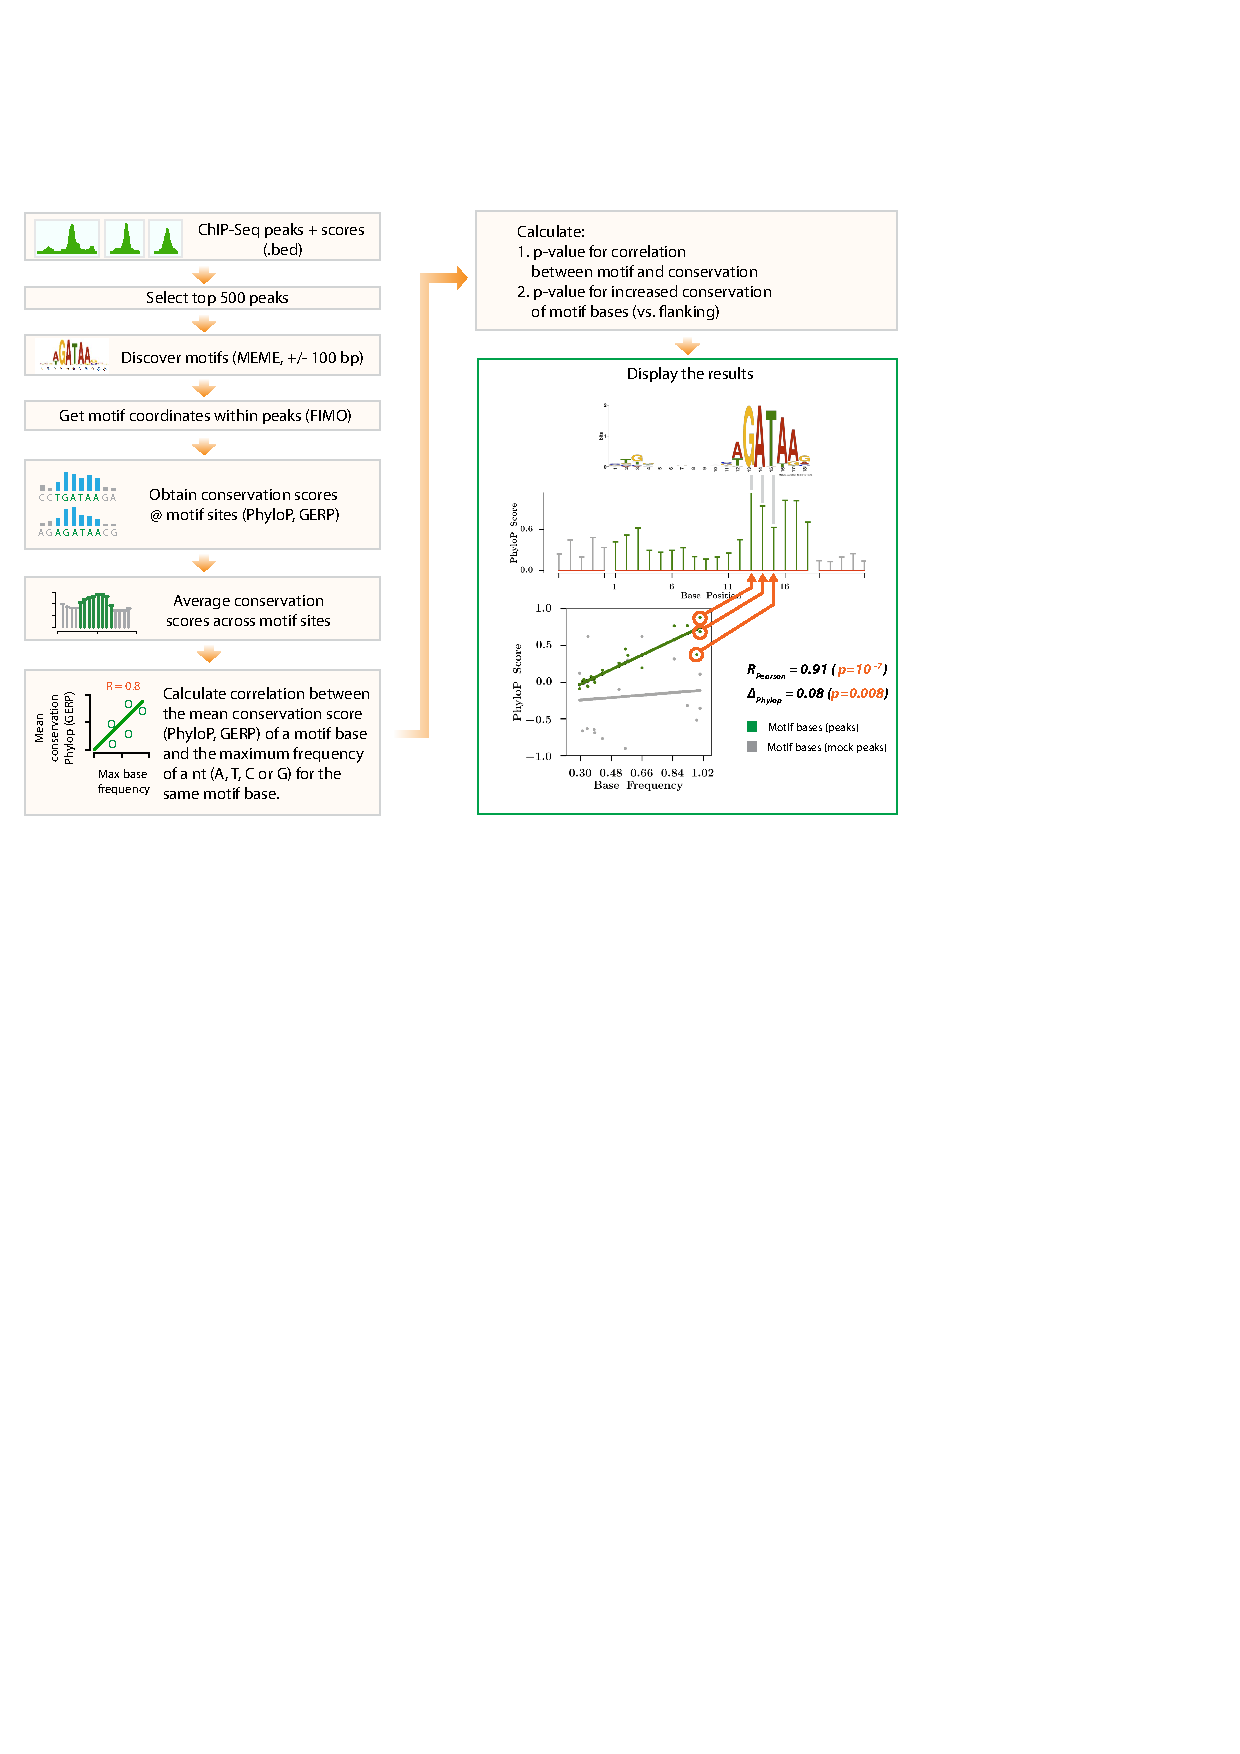
\includegraphics[width=0.9\linewidth]{workflow}
\captionof{figure}{MoCA Workflow}
\end{center}
%------------------------------------------------


}
\headerbox{References}{name=references,column=2, below=conclusion}{

\smaller % Reduce the font size in this block
\renewcommand{\section}[2]{\vskip 0.05em} % Get rid of the default "References" section title
\nocite{*} % Insert publications even if they are not cited in the poster

\bibliographystyle{unsrt}
\bibliography{abstract} % Use sample.bib as the bibliography file
\vspace{1em}

}
\vspace*{20em}

\includegraphics[scale=0.3]{usclogo}
\hspace{245pt}

\includegraphics[scale=0.15]{MoCA_Figshare}
%----------------------------------------------------------------------------------------

\end{poster}
\end{document}